\documentclass[fleqn]{article}
\oddsidemargin 0.0in
\textwidth 6.0in
\thispagestyle{empty}
\usepackage{import}
\usepackage{amsmath}
\usepackage{graphicx}
\usepackage{flexisym}
\usepackage{calligra}
\usepackage{amssymb}
\usepackage{bigints} 
\usepackage[english]{babel}
\usepackage[utf8x]{inputenc}
\usepackage{float}
\usepackage[colorinlistoftodos]{todonotes}


\DeclareMathAlphabet{\mathcalligra}{T1}{calligra}{m}{n}
\DeclareFontShape{T1}{calligra}{m}{n}{<->s*[2.2]callig15}{}
\newcommand{\scriptr}{\mathcalligra{r}\,}
\newcommand{\boldscriptr}{\pmb{\mathcalligra{r}}\,}

\definecolor{hwColor}{HTML}{691F80}

\begin{document}

  \begin{titlepage}

    \newcommand{\HRule}{\rule{\linewidth}{0.5mm}}

    \center

    \begin{center}
      
\includegraphics[height=11cm, width=11cm]{asu.png}
    \end{center}

    \vline

    \textsc{\LARGE Classical Parts/Field/Matter III}\\[1.5cm]

    \HRule \\[0.5cm]
    { \huge \bfseries Homework One}\\[0.4cm] 
    \HRule \\[1.0cm]

    \textbf{Behnam Amiri}

    \bigbreak

    \textbf{Prof: Samuel Teitelbaum}

    \bigbreak

    \textbf{{\large \today}\\[2cm]}

    \vfill

  \end{titlepage}

  \begin{enumerate}
    \item \textbf{(8.2. 15 pts)} Consider the charging capacitor in Prob. 7.34
    \begin{enumerate}
      \item Find the electric and magnetic fields in the gap, as functions of the distance $s$
      from the axis and the time $t$. (Assume the charge is zero at $t=0$.)

        \textcolor{hwColor}{
          \\
          Consider the charging capacitor below (Prob. 7.34)
        }

        \begin{center}
          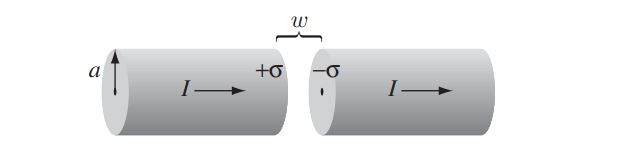
\includegraphics[height=3cm, width=10cm]{problem734.JPG}
        \end{center}

        \textcolor{hwColor}{
          Think of a single sheet that has a positive charge distributed through its surface and 
          consider a Gaussian surface in the form of a cylinder right in the middle of the sheet. Gaussian cylinder
          is going to emit an electric field that exists the cylinder in both directions. (Outward flux)
          We can calculate the electric field using the Gauss'a law: 
          \\
          \\
          $
            \bigoint E.da=\dfrac{1}{\epsilon_0} Q_{enc}
          $
          \\
          \\
          The Total electric flux for both siders of the Gaussian cylinder is $EA$. Therefore, $EA+EA=\dfrac{1}{\epsilon_0} Q$.
          We also know that surface charge density is $\sigma=\dfrac{Q}{A}$, so we have:
          \\
          $
            2EA=\dfrac{1}{\epsilon_0} \sigma A \Longrightarrow \overrightarrow{E}=\dfrac{\sigma}{2 \epsilon_0} \hat{z}
          $
          ~~~~~~ (Assuming the $\hat{z}$ is to the right)
          \\
          \\
          We now know the electric field of one plate then the electric field in between the two plates is:
          \\
          \\
          $
            \overrightarrow{E}+\overrightarrow{E}=\dfrac{\sigma}{2 \epsilon_0} \hat{z}+\dfrac{\sigma}{2 \epsilon_0} \hat{z}
            \\
            \\
            \\
            \therefore ~~~ \overrightarrow{E}=\dfrac{\sigma}{\epsilon_0} \hat{z}
          $
          \\
          \\
          Note: We assumed the charged is distributed uniformly. For a circular plate we have:
          \\
          \\
          $
            \sigma=\dfrac{Q}{A}=\dfrac{I ~ t}{\pi a^2}
            \\
            \\
            \\
            \therefore ~~~ \overrightarrow{E}=\dfrac{I ~ t}{\epsilon_0 \pi a^2} \hat{z} ~~~~ \checkmark
          $
          \\
          \\
          \\
          \\
          \\
          We can use the Ampere's law to find the magnetic field in the gap at a distance $s < a$. 
          \\
          \\
          $
            \bigoint B.dl=\mu_0 I_{enc}
            \\
            \\
          $
          In chapter 7, we learned about displacement current $J_d \equiv \epsilon_0 \dfrac{\partial E}{\partial t}$.
          Through the gap the displacment is in the $z$ direction. By rewriting the Ampere's law we have:
          \\
          \\
          $
            \bigoint B.dl=\mu_0 I_{dis} \Longrightarrow B \times 2 \pi s=\mu_0 I_{dis}
            \\
            \\
            I_{dis}=\bigints J_d.da
            =\bigints \left(\epsilon_0 \dfrac{\partial E}{\partial t}\right).da
            =\bigints\limits_{0}^{s} \bigints\limits_{0}^{2 \pi} \left[
              \epsilon_0 \dfrac{\partial}{\partial t} \left(\dfrac{I ~ t}{\epsilon_0 \pi a^2} \hat{z} \right)
            \right].s ~ ds ~ d\phi ~ \hat{z}
            \\
            \\
            =\bigints\limits_{0}^{s} \bigints\limits_{0}^{2 \pi} \left( 
              \dfrac{\epsilon_0 ~ I}{\epsilon_0 \pi a^2} \hat{z} 
            \right).s ~ ds ~ d\phi ~ \hat{z}
            =\left[\dfrac{I ~ s^2}{2 \pi a^2}\right]_{0}^{s} \times \left[2 \pi\right]
            \\
            \\
            \\
            \therefore ~~~ I_{dis}=\dfrac{I ~ s^2}{a^2} \Longrightarrow B \times 2 \pi s=\mu_0 I_{dis}=\mu_0 \dfrac{I ~ s^2}{a^2}
            \\
            \\
            \\
            \therefore ~~~ \overrightarrow{B}=\mu_0 \dfrac{I ~ s}{2 \pi a^2} \hat{\phi} ~~~~ \checkmark
          $
        }

      \item Find the energy density $u_{em}$ and the Poynting vector $S$ in the gap. Note especially 
      the direction of $S$. Check that $Eq. 8.12$ is satisfied.

        \textcolor{hwColor}{
          \\
          Eq 8.5 gives the energy density as (energy density)
          \\
          \\
          $
            u_{em}=\dfrac{1}{2} \left(\epsilon_0 E^2 + \dfrac{1}{\mu_0} B^2\right)
            =\dfrac{1}{2} \left(\epsilon_0  \dfrac{I^2 ~ t^2}{\epsilon_0^2 \pi^2 a^4} + \dfrac{1}{\mu_0}  \mu_0^2 \dfrac{I^2 ~ s^2}{4 \pi^2 a^4} \right)
            =\dfrac{1}{2} \left(\dfrac{I^2 ~ t^2}{\epsilon_0 \pi^2 a^4} + \dfrac{\mu_0 I^2 ~ s^2}{4 \pi^2 a^4} \right)
            \\
            \\
            \\
            \therefore ~~~ u_{em}=\dfrac{I^2}{2\pi^2 a^4} \left(\dfrac{t^2}{\epsilon_0} + \dfrac{\mu_0 s^2}{4} \right) ~~~~ \checkmark
            \\
            \\
          $
          The Poynting vector is defined in Griffiths as
          \\
          \\
          $
            \overrightarrow{S} \equiv \dfrac{1}{\mu_0} \left(E \times B\right)
            =\dfrac{1}{\mu_0} \left(
              \dfrac{I ~ t}{\epsilon_0 \pi a^2} \hat{z} 
              \times 
              \mu_0 \dfrac{I ~ s}{2 \pi a^2} \hat{\phi}
            \right)
            \\
            \\
            \\
            \therefore ~~~ \overrightarrow{S}=-\dfrac{I^2 t s}{2 \pi^2 \epsilon_0 a^4} \hat{s} ~~~~ \checkmark
          $
          \\
          \\
          The direction of $\overrightarrow{S}$ is in the $\hat{s}$ direction. We know that the direction of Poynting vector is 
          the direction of energy flow. Hence, the energy is flowing into the gap. Now we need to check that $Eq. 8.12$ is satisfied.
          $
            \dfrac{\partial u_{em}}{\partial t}=-\nabla.S  ~~~~~ Eq. 8.12.
            \\
            \\
            \begin{cases}
              \dfrac{\partial u_{em}}{\partial t}
              =\dfrac{\partial}{\partial t} \left[\dfrac{I^2}{2\pi^2 a^4} \left(\dfrac{t^2}{\epsilon_0} + \dfrac{\mu_0 s^2}{4} \right)\right]
              =\dfrac{I^2 t}{\pi^2 a^4 \epsilon_0}
              \\
              \\
              -\nabla.S=-\dfrac{1}{s} \dfrac{\partial}{\partial s} \left(s S\right)
              =-\dfrac{1}{s} \dfrac{\partial}{\partial s} \left(-s \dfrac{I^2 t s}{2 \pi^2 \epsilon_0 a^4}\right)
              =\dfrac{I^2 t}{\pi^2 \epsilon_0 a^4}
            \end{cases} \Longrightarrow \dfrac{\partial u_{em}}{\partial t}=-\nabla.S ~~~~ \checkmark
          $
          \\
          \\
          \\
          As we just saw, $Eq. 8.12$ holds. 
        }


      \item Determine the total energy in the gap, as a function of time. Calculate the total
      power flowing into the gap, by integrating the Poynting vector over the appropriate surface. 
      Check that the power input is equal to the rate of increase of energy in the gap ($Eq. 8.9$—in 
      this case $W=0$, because there is no charge in the gap). [If you’re worried about the fringing 
      fields, do it for a volume of radius $b < a$ well inside the gap.]

        \textcolor{hwColor}{
          \\
          $
            \dfrac{d W}{dt}=-\dfrac{d}{dt} \bigints\limits_{v} \dfrac{1}{2} \left(\epsilon_0 E^2+\dfrac{1}{\mu_0}B^2 \right) d\tau
            -\dfrac{1}{\mu_0} \bigoint\limits_{S} \left(E \times B\right).da
          $
          \\
          Previously, we found the energy density $u_{em}$. And we learned $Eq. 8.9$ (above) has two parts, is known
          as Poynting's theorem. The first integral on the right is the total energy stored in the fields.
          \\
          Since we have the energy density in the gap, we can use the first integral on the right side of the above equation to 
          calculate the total energy.
          \\
          \\
          $
            U=\bigints\limits_{v} \dfrac{1}{2} \left(\epsilon_0 E^2+\dfrac{1}{\mu_0}B^2 \right) d\tau
            =\bigints\limits_{0}^{a} \bigints\limits_{0}^{2 \pi} \bigints\limits_{0}^{w} 
            \dfrac{1}{2} \left(\epsilon_0 \dfrac{I^2 ~ t^2}{\epsilon_0^2 \pi^2 a^4}+\dfrac{1}{\mu_0} \mu_0^2 \dfrac{I^2 ~ s^2}{4 \pi^2 a^4} \right) s ~ ds ~ d\phi ~ dz
            \\
            \\
            \\
            =\dfrac{1}{2} \bigints\limits_{0}^{a} \bigints\limits_{0}^{2 \pi} \bigints\limits_{0}^{w} 
            \left(
              \dfrac{I^2 ~ t^2}{\epsilon_0 \pi^2 a^4}
              +\dfrac{\mu_0 I^2 ~ s^2}{4 \pi^2 a^4} 
            \right) s ~ ds ~ d\phi ~ dz
            =\dfrac{I^2}{2 \pi^2 a^4} \left(\dfrac{t^2 a^2}{2 \epsilon_0}+\dfrac{\mu_0 a^4}{16}\right) \left(2 \pi\right) \left(w\right)
            \\
            \\
            \\
            \therefore ~~~ U=\dfrac{I^2 w}{2 \pi a^2} \left(\dfrac{t^2}{\epsilon_0}+\dfrac{\mu_0 a^2}{8}\right) ~~~~ \checkmark
          $
          \\
          \\
          Now it's time to calculate the total power flowing into the gap, by integrating the Poynting vector
          over the appropriate surface as we are asked. The gap is cylindrical and the power flowing into the gap 
          is the closed surface integral $ \bigoint\limits_{S} S.da$. The Poynting vector points radially inward
          so the only contribution to this integral is from the cylindrical body of the capacitor. In other words
          the surface enclosing the cylindrical gap includes the circular surfaces at each of the plates but for the 
          two plates $S.da=0$, therefore they are not part of the solution.
          \\
          \\
          $
            P_{Gap}=\bigints\limits_{0}^{2 \pi} \bigints\limits_{0}^{w} S.\left(s ~ d\phi ~ dz ~ \hat{s} \right)
            =\bigints\limits_{0}^{2 \pi} \bigints\limits_{0}^{w} 
            \left(-\dfrac{I^2 t s}{2 \pi^2 \epsilon_0 a^4} \hat{s}\right).\left(s ~ d\phi ~ dz ~ \hat{s}\right)
            \\
            \\
            =\bigints\limits_{0}^{2 \pi} \bigints\limits_{0}^{w} 
            -\dfrac{I^2 t s^2}{2 \pi^2 \epsilon_0 a^4} ~ d\phi ~ dz
            =-\dfrac{I^2 t s^2}{2 \pi^2 \epsilon_0 a^4} \bigints\limits_{0}^{2 \pi} \bigints\limits_{0}^{w} ~ d\phi ~ dz
            =-\dfrac{I^2 t a^2}{2 \pi^2 \epsilon_0 a^4} \left(2 \pi w\right)
            \\
            \\
            \\
            \therefore ~~~ P_{Gap}=-\dfrac{I^2 t w}{\pi \epsilon_0 a^2}
          $
          \\
          \\
          Note: For the above calculation $s=a$. We are also asked to check that the power input is equal to the rate
          of increase of energy in the gap ($Eq.8.9$—in this case $W=0$, because there is no charge in the gap).
          \\
          \\
          $
            \dfrac{d W}{dt}=-\dfrac{d}{dt} \bigints\limits_{v} \dfrac{1}{2} \left(\epsilon_0 E^2+\dfrac{1}{\mu_0}B^2 \right) d\tau
            -\dfrac{1}{\mu_0} \bigoint\limits_{S} \left(E \times B\right).da
          $
          \\
          \\
          $\dfrac{d W}{dt}$ is zero simply because ther are no charges in the gap. Hence:
          \\
          \\
          $
            0=-\dfrac{d}{dt} \bigints\limits_{v} \dfrac{1}{2} \left(\epsilon_0 E^2+\dfrac{1}{\mu_0}B^2 \right) d\tau
            -\dfrac{1}{\mu_0} \bigoint\limits_{S} \left(E \times B\right).da
            \\
            \\
            \dfrac{d}{dt} \bigints\limits_{v} \dfrac{1}{2} \left(\epsilon_0 E^2+\dfrac{1}{\mu_0}B^2 \right) d\tau
            =-\dfrac{1}{\mu_0} \bigoint\limits_{S} \left(E \times B\right).da
            \\
            \\
            \dfrac{dU}{dt}=-\bigoint\limits_{S} S.da
            \\
            \\
            \dfrac{d}{dt} \left[\dfrac{I^2 w}{2 \pi a^2} \left(\dfrac{t^2}{\epsilon_0}+\dfrac{\mu_0 a^2}{8}\right)\right]
            =-\left[-\dfrac{I^2 t w}{\pi \epsilon_0 a^2}\right]
            \Longrightarrow
            \dfrac{I^2 t w}{\pi \epsilon_0 a^2}
            =\dfrac{I^2 t w}{\pi \epsilon_0 a^2}
            \\
            \\
            \\
            \therefore ~~~ \dfrac{dU}{dt}=-\bigoint\limits_{S} S.da ~~~~\checkmark
          $
        }
      
    \end{enumerate}

    \pagebreak

    \item \textbf{(8.4. 15 pts)}
    \begin{enumerate}
      \item Consider two equal point charges $q$, separated by a distance $2a$. Construct the
      plane equidistant from the two charges. By integrating Maxwell’s stress tensor
      over this plane, determine the force of one charge on the other.

        \begin{center}
          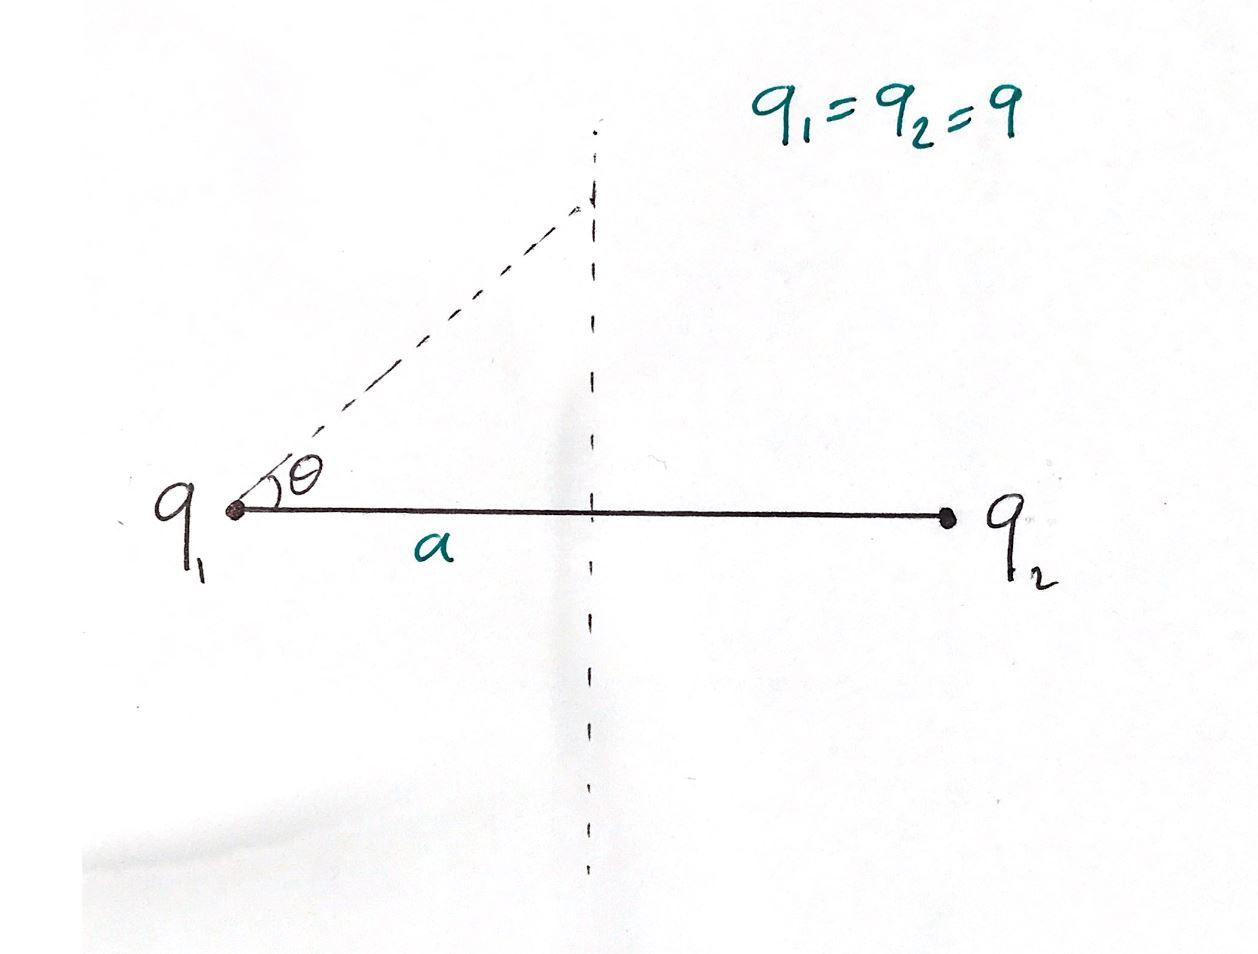
\includegraphics[height=6cm, width=10cm]{problem8.14.JPG}
        \end{center}

        \textcolor{hwColor}{
          \\
          On page 364 of the textbook we learned that the total electromagnetic force on the charges in $\mathcal{V}$ is
          \\
          \\
          $
            F=\bigoint\limits_{S} \overleftrightarrow{T}.da-\epsilon_0 \mu_0 \dfrac{d}{dt} \bigints\limits_{v} S d\tau
          $
          \\
          \\
          Note that We do not have magnetic fields in this problem. The \textbf{Maxwell Stress Tensor} is defined as 
          \\
          \\
          $
            T_{ij} \equiv \epsilon_0 \left(E_i E_j - \dfrac{1}{2} \delta_{ij} E^2 \right)
            +\dfrac{1}{\mu_0} \left(B_i B_j - \dfrac{1}{2} \delta_{ij} B^2\right)
            \\
            \\
            \\
            \therefore ~~~ \overleftrightarrow{T}=\epsilon_0 \begin{pmatrix}
              E_x^2-\dfrac{E^2}{2} && E_x E_y && E_x E_z
              \\
              E_y E_x && E_y^2-\dfrac{E^2}{2} && E_y E_z
              \\
              E_z E_x && E_z E_y && E_z^2-\dfrac{E^2}{2}
            \end{pmatrix}
          $
          \\
          \\
          We have two charges, let's call them charges 1 and 2. The force that charge 1 exerts on charge 2 is what we are 
          interested in. Imagine a system where the origin of it is on charge 1. Then the electric field due to charge 1
          is
          \\
          \\
          $
            E_1=\dfrac{q}{4 \pi \epsilon_0 r^2} \hat{r}
            =\dfrac{q}{4 \pi \epsilon_0} \left(\dfrac{1}{a^2+y^2+z^2}\right)
            \left(\dfrac{-a \hat{x}+y\hat{y}+z\hat{z}}{\sqrt{a^2+y^2+z^2}}\right)
          $
          \\
          The electric field of charge 2 is
          \\
          \\
          $
            E_2=\dfrac{q}{4 \pi \epsilon_0} \left(\dfrac{1}{(-a+2a)^2+y^2+z^2}\right)
            \left(\dfrac{(-a+2a) \hat{x}+y\hat{y}+z\hat{z}}{\sqrt{(-a+2a)^2+y^2+z^2}}\right)
            \\
            \\
            E_2=\dfrac{q}{4 \pi \epsilon_0} \left(\dfrac{1}{a^2+y^2+z^2}\right)
            \left(\dfrac{a \hat{x}+y\hat{y}+z\hat{z}}{\sqrt{a^2+y^2+z^2}}\right)
          $
          \\
          \\
          \\
          The total electric field between the charges is 
          \\
          \\
          $
            E=E_1+E_2
            =\dfrac{q}{4 \pi \epsilon_0} \left(\dfrac{1}{a^2+y^2+z^2}\right)
            \left(\dfrac{-a \hat{x}+y\hat{y}+z\hat{z}}{\sqrt{a^2+y^2+z^2}}\right)
            +\dfrac{q}{4 \pi \epsilon_0} \left(\dfrac{1}{a^2+y^2+z^2}\right)
            \left(\dfrac{a \hat{x}+y\hat{y}+z\hat{z}}{\sqrt{a^2+y^2+z^2}}\right)
            \\
            \\
            \\
            \therefore ~~~ E=\dfrac{q}{2\pi \epsilon_0} \left[\dfrac{1}{\left(a^2+y^2+z^2\right)^{3/2}}\right] \left[y \hat{y}+z \hat{z}\right] ~~~~ \checkmark
            \\
            \\
            \\
            \therefore ~~~ \begin{cases}
              E_x=0
              \\
              \\
              E_y=\dfrac{q}{2\pi \epsilon_0} \left[\dfrac{y}{\left(a^2+y^2+z^2\right)^{3/2}}\right]
              \\
              \\
              E_z=\dfrac{q}{2\pi \epsilon_0} \left[\dfrac{z}{\left(a^2+y^2+z^2\right)^{3/2}}\right]
              \\
              \\
              E^2=\dfrac{q^2}{4 \pi^2 \epsilon_0^2} \left[\dfrac{y^2+z^2}{\left(a^2+y^2+z^2\right)^3}\right]
            \end{cases}
          $
          \\
          \\
          Now, by getting back to the total electromagnetic force on the charges formula that was written 
          above, we can find the force on charge 2 due tio charge 1.
          \\
          \\
          $
            F=\bigints\limits_{-\infty}^{+\infty} \bigints\limits_{-\infty}^{+\infty} \overleftrightarrow{T}.dy ~ dz ~ \hat{x}
            \\
            \\
            \\
            \overleftrightarrow{T}.\hat{x}=\epsilon_0 \begin{pmatrix}
              -\dfrac{E^2}{2} && 0 && 0
              \\
              0 && E_y^2-\dfrac{E^2}{2} && E_y E_z
              \\
              0 && E_z E_y && E_z^2-\dfrac{E^2}{2}
            \end{pmatrix} \begin{pmatrix}
              1
              \\
              0
              \\
              0
            \end{pmatrix}
            =-\epsilon_0 \dfrac{E^2}{2} \hat{x}=-\dfrac{\epsilon_0}{2} \left[\dfrac{q^2}{4 \pi^2 \epsilon_0^2} \left[\dfrac{y^2+z^2}{\left(a^2+y^2+z^2\right)^3}\right]\right] \hat{x}
            \\
            \\
            \\
            \therefore ~~~ \overleftrightarrow{T}.\hat{x}=-\dfrac{q^2}{8 \pi^2 \epsilon_0} 
            \left[
              \dfrac{y^2+z^2}{\left(a^2+y^2+z^2\right)^3}
            \right] \hat{x} ~~~~ \checkmark
          $
          \\
          \\
          Plugging in $\overleftrightarrow{T}.\hat{x}$ into $F$ we get
          \\
          \\
          $
            F=\bigints\limits_{-\infty}^{+\infty} \bigints\limits_{-\infty}^{+\infty} \overleftrightarrow{T}.dy ~ dz ~ \hat{x}
            =\bigints\limits_{-\infty}^{+\infty} \bigints\limits_{-\infty}^{+\infty} \left[
              -\dfrac{q^2}{8 \pi^2 \epsilon_0} \left(\dfrac{y^2+z^2}{\left(a^2+y^2+z^2\right)^3}\right)
            \right].dy ~ dz ~ \hat{x}
            \\
            \\
          $
          Assuming the $yz$ plane be in cylindrical coordinates and $s=\sqrt{y^2+z^2}$ then
          \\
          \\
          $  
            =-\bigints\limits_{0}^{+\infty} \bigints\limits_{0}^{2 \pi} \dfrac{q^2}{8 \pi^2 \epsilon_0} \left(\dfrac{s^2}{(a^2+s^2)^3}\right) s ~ ds ~ d\phi ~ \hat{x}
            \\
            \\
            \\
            \bigints\limits_{0}^{+\infty} \dfrac{s^3}{\left(a^2+s^2\right)^3} ds \longrightarrow \begin{cases}
              u=s^2
              \\
              du=2s ds
            \end{cases}
            \\
            \\
            \\
            \therefore ~~~ \bigints\limits_{0}^{+\infty} \dfrac{s^3}{\left(a^2+s^2\right)^3} ds=\bigints\limits_{0}^{+\infty} \dfrac{s \times u}{\left(a^2+s^2\right)^3} \dfrac{du}{2s}
            =-\dfrac{1}{2} \left[\dfrac{u}{(u+a^2)^2}+\dfrac{a^2}{2(a^2+u)^2}\right]_{0}^{\infty}=\dfrac{1}{4a^2}
            \\
            \\
            \\
            F=-\bigints\limits_{0}^{+\infty} \bigints\limits_{0}^{2 \pi} \dfrac{q^2}{8 \pi^2 \epsilon_0} \left(\dfrac{s^2}{(a^2+s^2)^3}\right) s ~ ds ~ d\phi ~ \hat{x}
            =-\dfrac{q^2}{8 \pi^2 \epsilon_0} \dfrac{1}{4a^2} 2 \pi ~ \hat{x}
            \\
            \\
            \\
            \therefore ~~~ F=-\dfrac{q^2}{4 \pi \epsilon_0 (2a)^2} ~ \hat{x} ~~~~ \checkmark
          $
          \\
          \\
          This is the exact same result that we get if were to use the Coulomb's law.
          \\
        }


      \item Do the same for charges that are opposite in sign.
      
        \textcolor{hwColor}{
          \\
          Now one of the charges has to have opposite charge. The steps are the pretty much the same. 
          \\
          \\
          $
            E_1=\dfrac{q}{4 \pi \epsilon_0 r^2} \hat{r}
            =\dfrac{q}{4 \pi \epsilon_0} \left(\dfrac{1}{a^2+y^2+z^2}\right)
            \left(\dfrac{-a \hat{x}+y\hat{y}+z\hat{z}}{\sqrt{a^2+y^2+z^2}}\right)
            \\
            \\
            \\
            E_2=-\dfrac{q}{4 \pi \epsilon_0} \left(\dfrac{1}{a^2+y^2+z^2}\right) \left(\dfrac{a \hat{x}+y \hat{y}+z \hat{z}}{\sqrt{a^2+y^2+z^2}}\right)
            \\
            \\
            \therefore ~~~ E=E_1+E_2=\dfrac{q}{4 \pi \epsilon_0 \left(a^2+y^2+z^2\right)^{3/2}} \left(-2a \hat{x}\right)
            \\
            \\
            \overleftrightarrow{T}=\epsilon_0 \begin{pmatrix}
              \dfrac{E^2}{2} && 0 && 0
              \\
              0 && -\dfrac{E^2}{2} && 0
              \\
              0 && 0 && -\dfrac{E^2}{2}
            \end{pmatrix}
            \\
            \\
            \\
            \overleftrightarrow{T}.\hat{x}=\epsilon_0 \dfrac{E^2}{2} \hat{x}=\epsilon_0 \dfrac{4 a^2 q^2}{32 \pi^2 \epsilon_0^2 \left(a^2+y^2+z^2\right)^3} \hat{x}
            \\
            \\
            \\
            \therefore ~~~ \overleftrightarrow{T}.\hat{x}=\dfrac{a^2 q^2}{8 \pi^2 \epsilon_0 \left(a^2+y^2+z^2\right)^3} \hat{x}
            \\
            \\
            \\
            F=\bigints\limits_{-\infty}^{+\infty} \bigints\limits_{-\infty}^{+\infty} \dfrac{a^2 q^2}{8 \pi^2 \epsilon_0 \left(a^2+y^2+z^2\right)^3} dy dz
            \\
            \\
            =\bigints\limits_{0}^{+\infty} \bigints\limits_{0}^{2 \pi} \dfrac{a^2 q^2}{8 \pi^2 \epsilon_0 \left(a^2+s^2\right)^3} s ~ ds ~ d\phi ~ \hat{x}
            =\dfrac{a^2 q^2}{4 \pi \epsilon_0} \bigints\limits_{0}^{+\infty} \dfrac{s}{\left(a^2+s^2\right)^3} ds ~ \hat{x}
            =\left(\dfrac{a^2 q^2}{4 \pi \epsilon_0}\right) \left(\dfrac{1}{4a}\right) ~ \hat{x}
            \\
            \\
            \\
            \therefore ~~~ F=\dfrac{q^2}{4 \pi \epsilon_0 \left(2a\right)^2} ~ \hat{x} ~~~~ \checkmark
            \\
          $ 
        }
  
    \end{enumerate}


    \item \textbf{(8.16. 35 pts)} A sphere of radius $R$ carries a uniform polarization $P$ and a uniform
    magnetization $M$ (not necessarily in the same direction). Find the electromagnetic momentum of this configuration.
    [Answer: $\dfrac{4}{9} \pi \mu_0 R^3 (M \times P)$]
    

      % \textcolor{hwColor}{
      %   \\

      % }

    \item \textbf{(8.17. 35 pts)} Picture the electron as a uniformly charged spherical shell, with
    charge $e$ and radius $R$, spinning at angular velocity $\omega$.
    \begin{enumerate}
      \item Calculate the total energy contained in the electromagnetic fields.
      
        \textcolor{hwColor}{
          \\
          There was a similar question in chapter 5 where we found the magentic and electric fields inside and outside the shell as
          \\
          $
            \begin{cases}
              r>R \longrightarrow E=\dfrac{1}{4 \pi \epsilon_0} \dfrac{e}{r^2} \hat{r}, ~~ B=\dfrac{\mu_0 \sigma \omega R^4}{3 r^3} \left(2 cos(\theta) \hat{r}+sin(\theta) \hat{\theta}\right)
              \\
              \\
              r<R \longrightarrow E=0, ~~ B=\dfrac{2}{3} \mu_0 \sigma R \omega \hat{z}, ~~ \sigma=\dfrac{e}{4 \pi R^2}
            \end{cases}
            \\
            \\
          $
          \\
          We got the energy stored in the electric field
          \\
          \\
          $
            W_E=\dfrac{1}{8 \pi \epsilon_0} \dfrac{e^2}{R}
          $
          \\
          \\
          And the energy density of B as (inside)
          \\
          \\
          $
            u_B=\dfrac{1}{2 \mu_0} B^2=\dfrac{1}{2 \mu_0} \left(\dfrac{2}{3} \dfrac{\mu_0 R \omega e}{4 \pi R^2}\right)^2
            \\
            \\
            \\
            \therefore ~~~ W_{B_{inside}}=\dfrac{\omega^2 e^2 \mu_0 R^4}{18(16 \pi^2)} \dfrac{1}{r^6} \left(3 cos^2(\theta)+1\right)
          $
          \\
          \\
          And the energy density of B as (outside)
          \\
          \\
          $
            u_B=\dfrac{1}{2 \mu_0} \dfrac{\mu_0}{16 \pi^2} \dfrac{m^2}{r^6} \left(4 cos^2(\theta)+sin^2(\theta)\right)
            \\
            \\
            \\
            W_{B_{outside}}=\dfrac{\mu \omega^2 e^2 R^4}{288 \pi^2} \bigints\limits_{R}^{+\infty} \bigints\limits_{0}^{\pi} \bigints\limits_{0}^{2 \pi}
            \dfrac{1}{r^4} \left(3 cos^2(\theta)+1\right) sin(\theta) ~ dr ~ d\theta ~ d\phi
            \\
            \\
            =\dfrac{\mu_0 \omega^2 e^2 R^4}{288 \pi} \left(\dfrac{1}{3R^3}\right) \left(8 \pi\right)
            =\dfrac{\mu_0 \omega^2 e^2 R}{108 \pi}
            \\
            \\
            \\
            W=W_E+W_B=\dfrac{1}{8 \pi \epsilon_0} \dfrac{e^2}{R^2}+ \left[\dfrac{\mu_0 \omega^2 e^2 R}{108 \pi} \times 3\right]
            \\
            \\
            \\
            \therefore ~~~ W=\dfrac{1}{8 \pi \epsilon_0} \dfrac{e^2}{R^2}+\dfrac{\mu_0 \omega^2 e^2 R}{36 \pi} ~~~~ \checkmark
            \\
          $
        }

      \item Calculate the total angular momentum contained in the fields.
      
        \textcolor{hwColor}{
          \\
          $
            \begin{cases}
              m \longrightarrow \dfrac{1}{3} \omega e R^2
              \\
              \\
              Q \longrightarrow e
            \end{cases} \\Longrightarrow L=\dfrac{\mu_0 \omega e^2 R}{18 \pi} ~ \hat{z} ~~~~ \checkmark
            \\
          $
        }

      \item According to the Einstein formula $(E = mc^2)$, the energy in the fields should
      contribute to the mass of the electron. Lorentz and others speculated that the
      entire mass of the electron might be accounted for in this way: $U_{em} = m_e c^2$.
      Suppose, moreover, that the electron’s spin angular momentum is entirely
      attributable to the electromagnetic fields: $L_{em}=\dfrac{\hbar}{2}$. On these two 
      assumptions, determine the radius and angular velocity of the electron. What is their
      product, $\omega R$? Does this classical model make sense?

        \textcolor{hwColor}{
          \\
          $
            \dfrac{\hbar}{2}=\dfrac{\mu_0 \omega R e^2}{18 \pi} \Longrightarrow \omega R=\dfrac{9 \pi \hbar}{\mu_0 e^2}
            \\
            \\
            \\
            \therefore ~~~ \omega R=\dfrac{9 \pi \times 1.05 \times 10^{-34}}{\left(4 \pi \times 10^{-7}\right) \left(1.60 \times 10^{-19}\right)^2}
            =9.228 \times 10^{10} ~ m/s
            \\
            \\
            \\
            mc^2=\dfrac{1}{8 \pi \epsilon_0} \dfrac{e^2}{R} \left[1+\dfrac{2}{9}\left(\dfrac{\omega R}{c}\right)^2\right]
            =\dfrac{1}{8 \pi \epsilon_0} \dfrac{e^2}{R} \left[1+\dfrac{2}{9}\left(\dfrac{9.228 \times 10^{10}}{3 \times 10^8}\right)^2\right]
            =2.10 \times 10^4
            \\
            \\
          $
          \\
          Now we can find the radius $R$
          \\
          \\
          $
            \therefore ~~~ R=\dfrac{\left(2.10 \times 10^4\right) \left(1.6 \times 10^{-19}\right)^2}{8 \pi \left(8.85 \times 10^{-12}\right) \left(9.11 \times 10^{-31}\right) \left(3 \times 10^8\right)^2}
            =2.94 \times 10^{-11} ~ m ~~~~ \checkmark
            \\
            \\
            \\
            \therefore ~~~ \omega=\dfrac{9.228 \times 10^{10}}{R}=\dfrac{9.228 \times 10^{10}}{2.94 \times 10^{-11}}=3.1387 \times 10^{21} ~ rad/s ~~~~ \checkmark
          $
          \\
          \\
          This classical model does not make sense, simply because the value of $\omega R$ is insanely bigger than the speed of light.
          \\
        }
      
    \end{enumerate}


  \end{enumerate}

\end{document}
